\documentclass[10pt, conference, letterpaper]{IEEEtran}
\usepackage{cite}
\usepackage{xcolor,soul,framed}
\usepackage{amsmath,amsthm,amssymb,amsfonts}
\usepackage{algorithmic}
\usepackage{graphicx}
\usepackage{color, soul}
\usepackage{algorithm, algorithmic}
\usepackage[utf8]{inputenc}
\usepackage[english]{babel}
\usepackage{mathtools}
\graphicspath{ {./images/} }

%---------------------------------------------------------------%
\newtheorem{definition}{Definition}
\newtheorem{assumption}{Assumption}
\newtheorem{problem}{Problem}
\newtheorem{lemma}{Lemma}
\newtheorem{remark}{Remark}
\newtheorem{theorem}{Theorem}
\newtheorem{corollary}{Corollary}
\newtheorem{example}{Example}
\newcommand{\eq}{=}
\newcommand{\domZ}{\mathbb{Z}_{*}}
\newcommand{\vecOne}{\mathbf{1}}
\newcommand{\ind}{\mathbf{I}}
\newcommand{\mat}{\mathbf}
\newcommand{\define}{\triangleq}
\newcommand{\leadto}{\Rightarrow}
\renewcommand{\vec}{\mathbf}
\DeclarePairedDelimiter{\set}{\{}{\}}
\DeclarePairedDelimiter{\norm}{|}{|}
\DeclarePairedDelimiter{\Inorm}{\|}{\|_1}
\DeclarePairedDelimiter{\Paren}{\bigg(}{\bigg)}
\DeclarePairedDelimiter{\Bracket}{\bigg[}{\bigg]}
\DeclarePairedDelimiter{\Brace}{\bigg\{}{\bigg\}}
%---------------------------------------------------------------%
\newcommand{\apSet}{\mathcal{K}}
\newcommand{\esSet}{\mathcal{M}}
\newcommand{\jSpace}{\mathcal{J}}
\newcommand{\wSet}{\mathcal{W}}
\newcommand{\uSet}{\mathcal{U}}
\newcommand{\cSet}{\mathcal{C}}
\newcommand{\Stat}{\mathbf{S}}
\newcommand{\Obsv}{\mathcal{Y}}
\newcommand{\Policy}{\mathbf{\Omega}}
\newcommand{\ASpace}{\mathbf{A}}
%---------------------------------------------------------------%

\begin{document}
    %=============================== TITLE ===============================%
    \title{
        Obsolete Information-based Distributed Online Job Dispatching in Edge Computing System
    }
    \author{
        \IEEEauthorblockN{
            Yuncong Hong\IEEEauthorrefmark{1}\IEEEauthorrefmark{2},
            % Rui Wang\IEEEauthorrefmark{1},
            % Haisheng Tan\IEEEauthorrefmark{3},
            % Francis C.M. Lau\IEEEauthorrefmark{2}
        }
        \IEEEauthorblockA{
            \IEEEauthorrefmark{1}Southern University of Science and Technology, P.R. China,
            \IEEEauthorrefmark{2}The University of Hong Kong, Hong Kong,\\
            \IEEEauthorrefmark{3}University of Science and Technology of China, P.R. China
        }
    }
    \maketitle

    %============================== ABSTRACT ==============================%
    \begin{abstract}
        \label{sec:abstract}
        Edge computing is believed to be the solid solution for time-sensitive big data real-time calculation. The cooperation among edge servers in the system usually causes in-effective task scheduling due to obsolete information sharing which is hard to tackle.
        In this work, we formulate the problem with job dispatching in distributed Edge Computing system, and identify the difficulty exists in cooperation among AP nodes (Access Points) and ES nodes (Edge Servers) with delayed information. We design the broadcast information sharing scheme in the system and formulate the corresponding problem into a MDP problem. The value function approximation and one-step policy iteration method is adopted to obtain a sub-optimal dispatching policy whose performance can be bounded analytically.
    \end{abstract}

    % \begin{IEEEkeywords}
    %     Edge Computing, Job Dispatch, Delayed Information, Collective Observability, Distributed Multi-agent MDP
    % \end{IEEEkeywords}

    %============================ INTRODUCTION ============================%
    \begin{section}{INTRODUCTION}
        \label{sec:introduction}
        Edge computing is promising.
        \cite{Naha2018} is a survey about fog computing in latency-aware computing in IoT, and investigate numerous proposed computing architecture.
        In IoT (Internet of Things)/MAN (Metropolitan Area Network) scenario,

        Related works on job dispatching on scheduling in edge computing, mostly with centralized agent to apply action and seldom take delayed information impact into consideration.
        \hl{In the previous researches, there are many works investigated job dispatching strategies in the scenario of MEC.} Task Offloading Scenario:
        \begin{itemize}
            \item \text{[centralized, offloading, reduced state MDP]} \cite{Zheng2019} is a work considering maximizing the long-term utility in MEC offloading policy, and formulating the problem with MDP solved with Q-learning; \hl{(need long time online to converge to optimality, less performed than our proposed algorithm)}
            \item \cite{Du2018} propose an offline algorithm with MINLP problem formulation, considering min-max fairness guarantee in computation offloading and computation resource allocation in fog/edge computing scenario; \hl{with only one edge and one cloud node considered, so trivial}
            \item \cite{Alameddine2019} is a work considering task offloading, scheduling and resource allocation joint optimization with Benders Decomposition;
            \item \cite{Fan2017} considers cooperation of multiple MEC-BSs of computation offloading which minimizes total cost of time and energy consumption.
            \item \cite{ElHaber2019} is a work considers energy consumption for offloading in multi-tier edge clouds;
            \item \cite{Chen2018a} proposes joint optimization of task caching placement and offloading decision to achieve the lowest delay of task processing;
        \end{itemize}
        \hl{Different from previous work, we focus on out-of-dated information on decision making in multi-agent cooperation system. To our best knowledge, there are very limited discussions on this topic.}
        \begin{itemize}
            \item The earliest works on out-of-dated information we find is \cite{ref-01} (cited 167 times). In this work, the single agent is assumed not able to observe the global state, and thus they need communication to establish cooperation by sharing limited information. The agent considers communication as extra action to synchronize the states and thus incurs extra cost; \hl{(However, the communication is without delay, thus converted into POMDP problem)}
            \item The other work \cite{ref-02} considers continuous state observation with constant or stochastic delay with single agent;
            \item One researcher published a series of paper on this topic.
                \cite{Lyu2017} is work considering \emph{out-of-date knowledge} optimization in IoT computing scenario, with Lyapunov optimization;
                \text{[delay-sensitive, ToC]} \cite{Lyu2018} identify that task admission is critical to delay-sensitive applications in mobile edge computing, and proposes an (1-$\epsilon$)-approximation algorithm
                \text{[foggy, fully distributed online]} \cite{Lyu2018a} is a work fully distributed online optimization to minimize the time-average cost and achieve asymptotic optimality over infinite time;
                \cite{Lyu2018b} try to establish cooperation among selfish devices in fog computing, and out-of-date information is blamed for optimality gap but proved to asymptotically diminish with the proposed algorithm; \hl{(escape from the information but no use)}
        \end{itemize}
        % \item Service Placement Scenario:
            %     \begin{itemize}
                    % \item \cite{Rodrigues2017} is a work on minimizing service delay in mobile edge computing;
                    % \item \cite{Yang2016} is a work considering services placement and requests dispatching on edge servers, and leverage users' pattern to predict "service cache" for online decision making;
            %         \item \cite{Chen2018} is a work with SDN on task offloading and battery life saving, and solve the NLP problem with two sub-problems;
            %     \end{itemize}
            % \item With Game Theory:
            % \begin{itemize}
            %     \item \cite{yang2018} and \cite{Josilo2019a} considers distributed computation offloading game;
            %     \item \cite{Liu2018} is a work considering minimize users' power consumption with Lyapunov optimization and matching theory;
            %     \item \cite{Dinh2018} considers distributed multi-user offloading in wireless channel with selfish EPG (exact potential game);
            %     \item \cite{Josilo2019} considers selfish offloading to achieve Nash equilibrium;
            %     \item \cite{Chen2016} is a work considering multi-user computation offloading with multi-channel contention, and adopt game theory approach to achieve Nash equilibrium with upper bound of convergence time;
            %     \item \cite{Zhang2018} considers multi-user offloading under transmit power decision and user association decision;
            % \end{itemize}  
            % \item Misc:
                % \begin{itemize}
                    % \item \cite{Masip-Bruin2016} is a work with layered structure with foggy and cloud computation;
                    % \item  \cite{Guo2018} considers jointly offloading decision making and power allocation for UEs in SCNs (small-cell networks);
                    % \item \cite{Yu2018} is a system work published in ToMC, presents a framework to minimize remote execution overhead, and carry out real system experiments using large-scale data from cellular network provider.
                    % \item \cite{Wang2018} is a system work published in IEEE Access, considers the mobility of mobile users in limited coverage solved with service migration and handover, and propose a framework;
                % \end{itemize}

        We identify the delayed system information is unacceptable for explosion \emph{delay-sensitive jobs} in edge computing, and it's hard to establish cooperation among AP nodes because of obsolete information; identify that the uploading process affect the performance of heuristic greedy algorithm; identify that the delay-information sharing in decision making.

        In this article, we considers User Equipment offloaded jobs dispatching from Access Points to Edge Servers. \hl{(Why separate AP and ES)}
        The dispatching decision is applied on Access Points distributively but in a synchronize way with some prior stochastic knowledge.
        Information sharing for cooperation is designed via (aligned) broadcast, job dispatch decision should be made immediately based on the previous collective information;

        Our contributions:
        \begin{itemize}
            \item To our best knowledge, we are the first work to propose a MDP framework to characterize the obsolete information distributed decision and with performance bound;
            \item propose a instantaneous job dispatching scheme in a distributed cooperative way, with synchronized/asymptotical stochastic information;
            \item propose a global state MDP formulation to characterize the multi-agent problem;
            \item adopt value function approximation to reduce the traditional algorithm complexity, and come up with performance guarantee;
        \end{itemize}

        \hl{The remainder of this paper is organized as following.}
        In Sec.II, system model.
        In Sec.III, problem formulation.
        In Sec.IV, we introduce low-complexity MDP algorithm.
        In Sec.V, evaluation.
        In Sec.VI, conclusion.
    \end{section}

    %============================ SYSTEM MODEL ============================%
    \begin{section}{SYSTEM MODEL}
        \label{sec:model}
        \begin{subsection}{Network Model}
            We have access points (AP) and edge servers (ES) denoted as $\apSet \define \set{1,\dots,K}$ and $\mathcal{M} \define \set{1,\dots,M}$ respectively in our MEC (mobile edge computing) system depicted in Fig. \ref{fig:system}. In this system, we adopt the same timing mechanism at both AP and ES side with a minimum \emph{timeslot} lasting for $\tau$ seconds.

            \begin{figure}[ht]
                \centering
                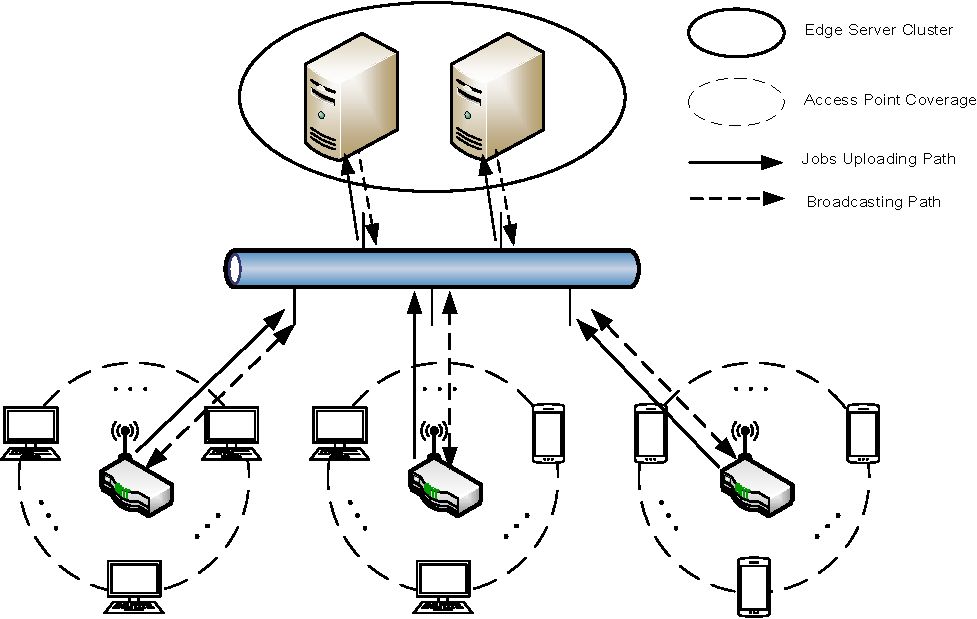
\includegraphics[width=0.45\textwidth, trim={0.5cm 0.5cm 0.5cm 0.5cm}, clip]{system-model.pdf}
                \caption{The Illustration of MEC System Model}
                \label{fig:system}
            \end{figure}

            The user equipment (UE) is connected to AP and offloads computation jobs to access point. Thus the job arrival process on $k$-th AP ($\forall k\in\apSet$) is compounded of the distributions from all UEs connected, which follows the assumption as:
            \begin{assumption}[Job Arrival Process for AP]
                The job arrival distribution for $k$-th AP is denoted as $A_k$, which is independent and identically distributed (i.i.d) over each timeslot as $A_k \sim Bernoulli(\lambda_k)$, $\lambda_k\in[0,1]$. This implies that there will be at most one job arrives on $k$-th AP in one timeslot. According to \emph{Poisson Limit Theorem}, the arrival process is a memory-less exponential process with average arrival rate $\mathbb{E}[A_k]=\lambda_k$.
                The jobs type distribution on each AP node follows the same distribution over job set $\jSpace$ which is obtained by statistics and denoted as $p_j \define \Pr\{\text{"j-type arrival"}\}$, where $\sum_{j\in\jSpace} p_j=1$.
            \end{assumption}

            The AP itself is assumed with no computation capability, and thus it need to further dispatch those jobs to the edge servers.
            The offloaded jobs on AP will be immediately dispatched to edge servers in each timeslot. The corresponding uploading delay of one job is {\color{red}deterministic and job-type dependent} over one AP-ES link, which is denoted as $u_{k,m}(j)$ from $k$-th AP to $m$-th ES ($\forall k\in\apSet, \forall m\in\esSet$).
            The network topology between AP cluster and ES cluster is fully accessible so that AP could dispatch jobs to any ES nodes in this system.

            After arrival on edge servers, the jobs will join computation with the supported VM (Virtual Machine).
            For jobs computation on edge servers, we adopt \emph{unrelated machines} assumption in \cite{tan-online}, where the job processing time on different servers are machine dependent and variant of resource or VM (virtual machine) constraints.
            Moreover, we have $L_{m,j}$ to denote the processing time for $j$-type job on $m$-th edge serer following some distribution, whose largest processing time is bounded by $L_C$.
            For convenience, we assign type of jobs on edge servers which have no VM resource available with \emph{infinity} processing time, and this kind of dispatching possibility will be rejected at the AP side.

            Each VM is considered running paralleled without resource contention, and the job scheduling for each VM follows \emph{FCFS} (First-Come-First-Serve).
            {\color{red}The maximum queue length is set to discourage too many jobs pending on edge servers and is denoted as $L_Q$. The job submission over the limit will be rejected and announce the AP where the job is from.}
        \end{subsection}

        \begin{subsection}{Information-Sharing Broadcast Model}
            As there is no centralized agent design to distribute the dispatching decisions to each AP node, all the AP nodes have to collect the global information from other nodes. Therefore, a information sharing scheme is needed to facilitate efficient cooperation among standalone AP nodes.
            In this article, the sharing is designed via periodic broadcasting, where all the AP and ES nodes in the system should broadcast their system related information with a same period interval as $t_B$. More specifically, the broadcasting is applied in a synchronized way that all the nodes start to broadcast at the start of same timeslot and repeat broadcasting after the same periodic interval $t_B$. We call each periodic point of broadcasting as \emph{broadcast point} and denote the $i$-th broadcast with $t_i$ where,
            \begin{align}
                t_i = i \cdot t_B, i=0,1,2,\dots
            \end{align}
            For $i$-th \emph{broadcast point}, the composed broadcast information from all the AP and ES nodes, and the corresponding information is listed as following:
            \begin{itemize}
                \item The $k$-th AP ($\forall k\in\apSet$) contains information $\mat{R}_k(i) \define (r^{(k)}_{m,j}(i))_{\set{m\in\esSet,j\in\jSpace}}$, where $r^{(k)}_{m,j}(i)$ denotes the remaining number of $j$-type jobs in uploading to $m$-th ES at time $t_i$; and we have $\vec{r}^{(k)}_{m} \define (r^{(k)}_{m,j}(i))_{j\in\jSpace}$ to denote the rows in $\vec{R}_k(i)$; % and $\vec{\hat{r}}^{(k)}_{j}$ to denote the columns;
                \item The $m$-th ES ($\forall m\in\esSet$) contains information $\vec{Q}_m(i) \define \set{Q_{m,j}(i)|\forall j\in\jSpace}$ to denote the computation queues for different job types, where $Q_{m,j}(i) \define (n_{m,j}(i), \delta_{m,j}(i))$ to characterize the $j$-type FIFO queue on $m$-th ES; $n_{m,j}(i)$ denotes the number of $j$-type job queueing on $m$-th ES, and $\delta_{m,j}(i)$ denotes the remaining processing time for last job.
            \end{itemize}
            Thus the composed broadcasting information is denoted as:
            \begin{align}
                \Obsv_i \define
                        \Brace{
                            \set{\mat{R}_{k}(i)|\forall k\in\apSet},
                            \set{\vec{Q}_m(i)|\forall m\in\esSet}
                        },
            \end{align}
            where $\Obsv_i$ is a set of global information of $i$-th broadcast. And it's actually the global system states at $t_i$.

            {\color{red}Due to the unpredictable property of broadcast delay with the underlaid network topology, different AP nodes will receive the broadcast information from AP nodes or ES nodes with different stochastic delay. However, we still assume the broadcast delay is upper bounded and with a statistical distribution in this interval.}
            Let $d^{(p)}_{k,k'}$ denotes the broadcast delay between two AP nodes from $k'$-th AP to $k$-th AP ($\forall k,k'\in\apSet$); let $d^{(s)}_{k,m}$ denotes the broadcast delay between AP and ES node from $m$-th ES to $k$-th AP ($\forall k\in\apSet,\forall m\in\esSet$).
            
            The AP will update its dispatching policy when it receives the information from edge servers, and the time it receives all the information. We call the policy update time in the broadcast interval as \emph{update points}, which is defined as following:
            \begin{definition}[Hehehehehehehehehe]
                MAXIMUM BROADCAST DELAY Hah!
            \end{definition}

            As the update points for each AP is key knowledge for optimal policy generation in our proposed scheme in next section, we furthermore design another broadcast phase where the AP nodes should broadcast the exact \emph{update points} list to other nodes

            The broadcast design introduces a \emph{Two-time scale} structure in the MEC system.
            The job dispatching and scheduling decisions on AP and ES side respectively are still carried out based on timeslot scale, while jobs' status transition from uploaded to computation is based on broadcast interval.
            More specifically, we consider the uploaded jobs in current broadcast interval will keep waiting on edge servers, and join the computation queue for scheduling at the beginning of next broadcast interval.
            {\color{red}To discourage the meaningless waiting on edge servers, the servers will announce all the AP nodes with \emph{empty-queue-penalty} in next broadcast. Moreover, we implement the broadcast in a low-frequency way that the broadcast period is always larger than the maximum broadcast delay plus the maximum uploading delay, i.e. $t_B > \hat{d}_{k} + u_{k,m}(j)$ $(\forall k\in\apSet, \forall m\in\esSet)$.}
        \end{subsection}
    \end{section}

    %============================ FORMULATION =============================%
    \begin{section}{PROBLEM FORMULATION}
        \label{sec:formulation}
        In this section, we formulate the standard MDP problem with respect to the broadcast-point time scale. The formulated problem is based on global information shared via synchronized broadcast, and the the optimal solution is achieved via compounded dispatching policies on all AP nodes.
        Given the fact that AP nodes would obtain global states update only after \emph{maximum broadcast delay} in each broadcast interval, the formulated MDP problem is composed of two adjacent broadcast interval with obsolete information and updated information.
        Then we show that the solution for all AP nodes suffers from curse of dimensionality and a low-complexity solution is needed.

        \begin{subsection}{System State and Dispatching Policy}
            The system states is selected based on the nature that $k$-th AP comes up with complete broadcast information only after its corresponding \emph{maximum broadcast delay} in the broadcast interval.
            The relative difference between broadcast point and the maximum delay point is depicted in Fig. \ref{fig:br-trans} \hl{(need to modify the state denotation in figure)}.
            \begin{definition}[System State]
                The system state at $i$-th broadcast point is denoted as $\Stat_i \define (\Obsv_{i}, \Obsv_{i-1}), (i=1,2,\dots)$, where $\Obsv_{i-1}$ represents the obsolete information before the broadcast received, and $\Obsv_{i}$ represents the updated information after the corresponding $\hat{d}_k$ delay for $k$-th AP node.
            \end{definition}

            \begin{figure}[ht]
                \centering
                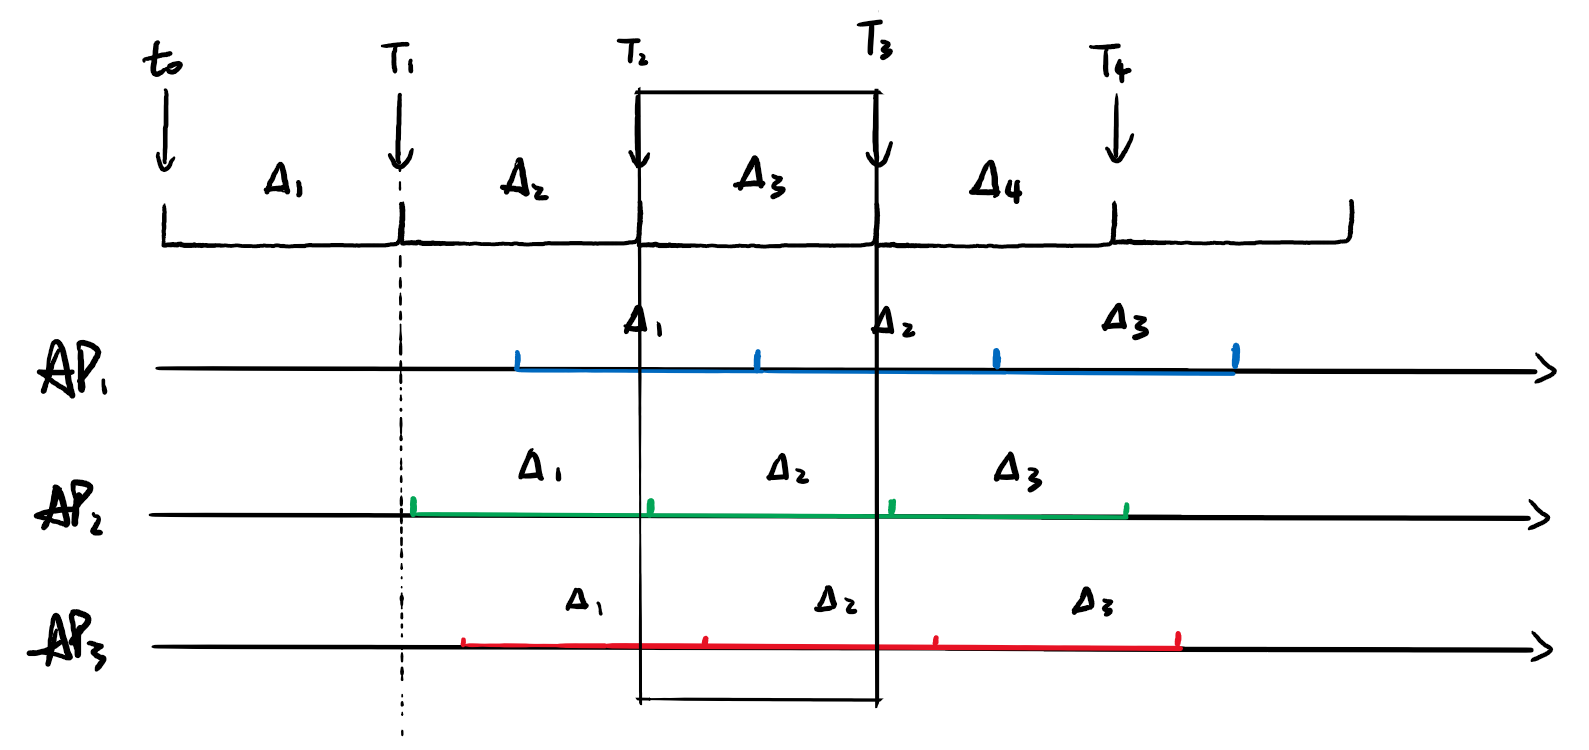
\includegraphics[width=0.45\textwidth]{broadcast-trans.png}
                \caption{Global Consensus and Transition with Delayed Action}
                \label{fig:br-trans}
            \end{figure}

            The \emph{dispatching policy} is applied over arrival jobs in each timeslot on each AP
            , and the \emph{dispatching action space} is defined as $\mathbf{A}: (j, m) \in \jSpace \times \esSet$, where $(j, m)$ denotes the action that $j$-type job should be uploaded to $m$-th ES.
            Based on the two stages of global system information $\Obsv_{i-1}$ and $\Obsv_{i}$ in system state, the compounded global-wise policy of all AP nodes is defined as following:
            \begin{definition}[Compounded Dispatching Policy]
                The compounded dispatching policy over $\Stat_{i}$ is defined as $\Policy(\Stat_{i})$ which is composed of all the local policies $\Omega_k(\Stat_{i})$ ($\forall k\in\apSet$) as:
                \begin{align}
                    \vec{\Omega}(\Stat_{i}) \define \Bracket{\Omega_1(\Stat_{i}), \dots, \Omega_K(\Stat_{i})}.
                \end{align}
                More specifically, $\Omega_k(\Stat_{i})$ is composed of two-stage policy as:
                \begin{align}
                    \Omega_k(\Stat_i) = [\tilde{\Omega}_k(\Obsv_{i-1}), \tilde{\Omega}_k(\Obsv_{i})],
                    % $t\in[t_{i-1}, t_{i}], \Delta{t} \define t - t_{i-1}$
                \end{align}
                where $\tilde{\Omega}_k(\Obsv_{i}) \define \set{\omega^{(i)}_{k,m}(j)|\forall j\in\jSpace, \forall m\in\esSet}$ and $\omega^{(i)}_{k,m}(j)$ denotes the dispatching policy that: based on global information $\Obsv_{i}$, the probabilistic action on $k$-th AP upload $j$-type job to $m$-th ES ($\sum_{j\in\jSpace} \Pr\{\omega^{(i)}_{k,m}(j)\}=1$).
            \end{definition}
            More specifically, the two phase of the policy on single AP is separated by the \emph{maximum broadcast delay} $\hat{d}_k$ to $k$-th AP, i.e. the time point when it receives the latest global information. For example, in the broadcast interval $[t_{i}, t_{i+1}]$, $k$-th AP will apply policy $\tilde{\Omega}_k(\Obsv_{i})$ based on obsolete information before maximum delay $\hat{d}_k$ and apply $\tilde{\Omega}_k(\Obsv_{i+1})$ immediately after the delay.
        \end{subsection}

        \begin{subsection}{The Optimization Problem}
            The optimization target of our problem is to minimize the \emph{average response time} of all jobs, which is composed of uploading time from AP to ES, and queueing-and-service time on ES nodes. According to \emph{Little's Law}, the average response time of all the jobs is equally as average number of jobs in system. Therefore, based on the system state definition, we have cost function as:
            \begin{align}
                g\Paren{\Stat_{i}, \Policy(\Stat_{i-1})} \define
                        \sum_{k\in\apSet}\sum_{m\in\esSet} \Inorm{\vec{r}^{(k)}_{m}(i)} +
                        \sum_{m\in\esSet}\sum_{j\in\jSpace} n_{m,j}(i),
            \end{align}
            where $\Inorm{\vec{r}^{(k)}_{m}}$ denotes the $L^1$-norm of vector $\vec{r}^{(k)}_{m}$, i.e. the sum up of absolute value of each entry. The cost function defined is a sampling of interval $t_B$ over the whole process, because the global information for AP nodes only contains the information at the broadcast points.

            Our distributed optimization problem definition is given as following:
            \begin{problem}[Distributed Cooperative Job Dispatching Problem]
                \begin{gather}
                    \min_{\Policy} \lim_{T \to \infty}
                        \mathbb{E}_{\Policy, \set{\hat{d}_k|\forall k\in\apSet}}
                            \Bracket{\sum_{i=2}^{T} \gamma^{i-1} g(\Stat_{i}, \Policy(\Stat_{i-1}))|\Stat_1},
                \end{gather}
                where the cost is collected with a discount factor $\gamma$.
            \end{problem}

            According to \cite{sutton1998introduction}, the above problem could be solved by the following \emph{Bellman's equation}:
            \begin{align}
                V(\Stat_{i}) =& g(\Stat_i)
                \nonumber\\
                &+ \gamma \min_{\Policy(\Stat_{i})} \sum_{\Stat_{i+1}} \sum_{\hat{d}_k} \Pr\{ \Stat_{i+1}|\Stat_{i}, \Policy(\Stat_{i}) \} V(\Stat_{i+1}),
            \end{align}
            where the original definition for value function defined in \cite{sutton1998introduction} is as following:
            \begin{align}
                V(\Stat_{i}) \define \lim_{T\to\infty}
                    \mathbb{E}_{\Policy}\Bracket{
                        \sum_{l=0}^{T} \gamma^l g\Paren{\Stat_{i+l}, \Policy(\Stat_{i+l-1})}
                    }.
            \end{align}

            Before diving into the analysis on the transition function expression, we firstly come up with some probability denotations for arrival process on edge servers.
            The job arrival processes for AP nodes under dispatching policy compose the job arrival process for ES nodes, which could be expressed as compounded of \emph{numbers arrival distribution} and \emph{processing time distribution} for $j$-type job ($\forall j\in\jSpace$).
            \begin{itemize}
                \item The \emph{numbers arrival distribution} on $m$-th ES is composed of i.i.d Bernoulli distribution in each timeslot from independent AP nodes. The PMF (probability mass function) of the Bernoulli distribution from $k$-th AP under policy $\Omega_k(i)$ is denoted as:
                \begin{align}
                    p_{k,m}^{(i)}(j) \define& \lambda_k p_j \cdot
                        \frac{
                                \Pr\{\omega_{k,m}^{(i)}(j)\}
                            }{
                                \sum_{j\in\jSpace} \Pr\{\omega_{k,m}^{(i)}(j)\}
                            },
                %     \\
                %     p_{k,m}^{(i)} \define& \sum_{j\in\jSpace} p_{k,m}^{(i)}(j),
                \end{align}
                and we have $\rho_{k,m}^{(\Pi_k)}$ denotes the distribution under time-invariant policy $\Pi_k$ for $k$-th AP;
                \item The \emph{processing time distribution} is job-independent, thus the processing time on different edge servers keeps its original distribution and is determined when the time it joins the processing queue.
            \end{itemize}
            
            \begin{lemma}[Transition Function Decoupling]
                The transition function in Bellman's equation could be decoupled to facilitate the final approximated value function expression. The transition function could be decoupled as:
                \begin{align}
                    & \Pr\{\Stat_{i+1}|\Stat_{i}, \Policy(\Stat_{i})\} 
                    \nonumber\\
                    =& \prod_{k\in\apSet} \Pr\Brace{\vec{R}_k(i+1)|\Policy(\Stat_{i})} \times \prod_{m\in\esSet}\prod_{j\in\jSpace}
                        \nonumber\\
                        & \Pr \Brace{\vec{Q}_{m,j}(i+1)|\vec{Q}_{m,j}(i), \set{\vec{R}_k(i)|\forall k\in\apSet}, \Policy(\Stat_{i})},
                \end{align}
                where first production part denotes the unfinished uploading state transition for AP nodes whose distribution, and the second part denotes the queueing state transition for ES nodes.
            \end{lemma}
            \begin{proof}
                Please refer to appendix \ref{trans-decouple}.
            \end{proof}

            As the formulated problem above is of infinite states and the action space would be exponentially expanded with respect to number AP and ES nodes, we could not use traditional \emph{policy iteration} or \emph{value iteration} algorithm \cite{sutton1998introduction} for unacceptable computational complexity. To alleviate curse of dimensionality, we take baseline dispatching policy to approximate the value function for each AP and ES nodes, and then carry out one-step iteration to obtain a better value function approximation.
        \end{subsection}
    \end{section}

    %============================= ALGORITHM ==============================%
    \begin{section}{LOW-COMPLEXITY SOLUTION}
        \label{sec:algorithm}
        In this section, we introduce a heuristic dispatching algorithm as the baseline policy, whose value function could be derived analytically. Then the joint expression with transition function as the optimization problem on right-hand side, we could further reduce the state complexity with averaged queueing dynamics on ES nodes.
        \hl{The proposed low-complexity sub-optimal policy can be obtained via the above approximated value function and one-step policy iteration. The derived value function becomes the cost upper bound of the proposed policy.}

        \begin{subsection}{Baseline Dispatching Policy}
            The baseline dispatching policy is adopted to obtain an approximation of value function. The policy on each AP nodes is randomized and time-invariant which is denoted as:
            \begin{align}
                \vec{\Pi} \define \Bracket{\Pi_1, \Pi_2, \dots, \Pi_K},
            \end{align}
            where $\Pi_k \define \set{\omega_{k,m}(j)|\forall m\in\esSet,\forall j\in\jSpace}$, $\forall k\in\apSet$.

            According to the linear property of cost function, the value function could be divided linearly into two section as $\tilde{W}^{(p)}(\Obsv^{(p)}(i))$ and $\tilde{W}^{(s)}(\Obsv(i))$ under baseline policy:
            \begin{align}
                V(\Stat_{i}) =& 
                    g(\Stat_{i}) + \gamma \min_{\Policy(\Stat_{i})} \sum_{\Stat_{i+1}} \Pr\{ \Stat_{i+1}|\Stat_{i}, \Policy(\Stat_{i}) \}
                    \nonumber\\
                    & \cdot \Bracket{ \tilde{W}^{(p)}\Paren{\Obsv^{(p)}(i+1)} + \tilde{W}^{(s)}\Paren{\Obsv(i+1)} },
            \end{align}
            where $\tilde{W}^{(p)}(\cdot)$ and $\tilde{W}^{(s)}(\cdot)$ denote the split value function over AP nodes and ES nodes respectively; $\Obsv^{(p)}(i) \define \set{\mat{R}_k(i)|\forall k\in\apSet}$ and $\Obsv^{(s)}(i) \define \set{\vec{Q}_m(i)|\forall m\in\esSet}$ respectively denote the AP states collection and ES states collection for $\Obsv(i) = \set{\Obsv^{(p)}(i), \Obsv^{(s)}(i)}$, and the split value function is in the following form:
            \begin{align}
                &\tilde{W}^{(p)}\Paren{\Obsv^{(p)}(i)} \define \sum_{k\in\apSet}\sum_{m\in\esSet}
                    \mathbb{E}_{\Pi}\Bracket{\sum_{l=0}^{\infty} \gamma^{l} \Inorm{\vec{r}^{(k)}_{m}(i+l)}}
                \\
                &\tilde{W}^{(s)}\Paren{\Obsv(i)} \define \sum_{m\in\esSet} \sum_{j\in\jSpace}
                    \mathbb{E}_{\Pi}\Bracket{\sum_{l=0}^{\infty} \gamma^{l} n_{m,j}(i+l)}
            \end{align}
            The decoupled value functions for AP and ES nodes is obtained with an approximated form under the baseline policy.

            The approximated value function $\tilde{W}^{(p)}(\Obsv^{(p)}(i+1))$ for AP nodes is obtained as:
            \begin{align}
                \tilde{W}^{(p)}(\Obsv^{(p)}(i+1)) = \frac{1}{1-\gamma}
                    \sum_{k\in\apSet}\sum_{m\in\esSet} \mathbb{E}_{\Pi}[\Inorm{\vec{r}^{(k)}_{m}}],
            \end{align}
            where the expectation of $\Inorm{\vec{r}^{(k)}_{m}}$ under the policy $\Pi_k$ is actually a constant as expectation of Binomial distribution $\mathbb{E}_{\Pi_k}[\Inorm{\vec{r}^{(k)}_{m}}] = \sum_{j\in\jSpace} u_{k,m} \rho^{(\Pi_k)}_{k,m}(j)$.
            
            The approximated value function $\tilde{W}^{(s)}(\Obsv(i))$ for ES nodes is affected with both arrival process under dispatching policy and last queue state, and we reduce the states expression by averaging the uploading process together with the transition function expression.
            % For convenience, we have $\Obsv^{(p)}(i) \define \set{\vec{u}_k(i)|\forall k\in\apSet}$ and $\Obsv^{(s)}(i) \define \set{Q_m(i)|\forall m\in\esSet}$.
            The partial value function optimization for ES in Bellman's Equation right-hand side is given as:
            \begin{align}
                \min_{\Policy(\Stat_i)}& \sum_{\Stat_{i+1}}
                    \Pr\Brace{\Stat_{i+1}|\Stat_{i}, \Policy(\Stat_i)} \cdot \tilde{W}^{(s)}\Paren{\Obsv(i+1)}
                \nonumber\\
                % \leadto \min_{\Policy(\Stat_i)}& \sum_{\Obsv^{(s)}(i)} \Pr\{\Obsv^{(s)}(i+1)|\Obsv^{(s)}(i),\Obsv^{(p)}(i), \Policy(\Stat_i)\}
                %     \nonumber\\
                %     & \times \sum_{\Obsv^{(p)}(i)} \Pr\{\Obsv^{(p)}(i+1)|\Policy(\Stat_i)\} \cdot \tilde{W}^{(s)}(\Obsv(i+1))
                % \nonumber\\
                = \min_{\Policy(\Stat_i)}& \sum_{\Obsv^{(s)}(i+1)}
                    \Pr\Brace{\Obsv^{(s)}(i+1)|\Obsv^{(s)}(i), \Obsv^{(p)}(i), \Policy(\Stat_i)}
                    \nonumber\\
                    \times& \sum_{m\in\esSet} \sum_{j\in\jSpace}
                        \underbrace{
                            \mathbb{E}_{\set{\Obsv^{(p)}(i+1)|\Policy(\Stat_i)}} \Bracket{\tilde{W}^{(s)}_{m,j}\Paren{\Obsv(i+1)}}
                        }_{
                            J\Paren{Q_{m,j}(i+1)}
                        },
            \end{align}
            where $\tilde{W}^{(s)}_{m,j}(\Obsv(i+1)) \define \mathbb{E}_{\Pi}[\sum_{l=0}^{\infty} \gamma^{l} n_{m,j}(i+l+1)]$, which implies that the state $\Obsv^{(p)}(i)$ is substitute with its expectation under policy $\Policy(\Stat_i)$ in this value function.
            Thus the approximated value function for $m$-th ES node is denoted as:
            \begin{align}
                J\Paren{Q_{m,j}(i+1)} \define& \lim_{T\to\infty}
                    \mathbb{E}_{\vec{\Pi}} \Bracket{\sum_{l=0}^{T} \gamma^{l} n_{m,j}(i+l+1)}
                \nonumber\\
                % =& \vec{u}'_i [\lim_{T\to\infty} \sum_{n=0}^{T} (\gamma \mat{P}_m)^{n}] \vec{g}_q
                % \nonumber\\
                =& \vec{\mu}'_i \Paren{ \mat{I}-\gamma\mat{P}_{m,j} }^{-1} \vec{g},
            \end{align}
            where $\vec{\mu}'_i$ denotes the transpose of $\vec{\mu}_i$, and $\vec{\mu}_i = [\dots,0,1,0,\dots]$ with only $i$-th element as $1$; the $i$-th element of $\vec{g}$ denotes the cost of server as $n_{m,j}(i)$ for $i$-th stage; $\mat{P}_{m,j}$ denotes the transition matrix for $j$-type FIFO queue on $m$-th ES under the policy $\vec{\Pi}$, which is composed of the following transition function ($\forall Q_m(i),Q_m(i+1)$) as:
            \begin{align}
                &\Pr \Brace{Q_{m,j}(i+1)|Q_{m,j}(i),\vec{\Pi}}
                \nonumber\\
                &=,
                % \begin{cases}
                %     I[\tilde{n}_{m,j}(i)L_{m,j}+\delta_{m,j}(i) \leq T_B], &\\
                %         \;\;\;\;\;\;\;\;\text{if } Q_{m,j}(i+1)=0,\delta_{m,j}(i+1)=0 \\
                %     I[\tilde{n}_{m,j}(i)L_{m,j}+\delta_{m,j}(i) > T_B] \times I[\delta_{m,j}(i+1)=\delta'_{m,j}(i)] 
                %     \nonumber\\
                %     \times I[\tilde{n}_{m,j}(i) - n'_{m,j}(i) = n_{m,j}(i+1)], &\\
                %         \;\;\;\;\;\;\;\;\text{otherwise}
                % \end{cases},
            \end{align}
            where:
            % \begin{itemize}
            %     \item $\tilde{n}_{m,j}(i) = \sum_{k\in\apSet} [\tilde{n}^{(k)}_{0,j} + \tilde{n}^{'(k)}_{m,j}] + n_{m,j}(i)$, where $\tilde{n}^{(k)}_{0,j} = u_{k,m}p^{(i)}_{k,m}(j)$ is the averaged $\Obsv^{(AP)}$ state under policy $\Policy(\Stat_i)$, $\tilde{n}^{'(k)}_{m,j} \sim B(t_B-u_{k,m}, p^{(\Pi_k)}_{k,m}(j))$, $(\forall k\in\apSet)$;
            %     \item $T_B+\delta_{m,j}(i)= n'_{m,j}(i) L_{m,j} + \delta'_{m,j}(i)$; if both $\delta_{m,j}(i+1)=0$ and $n_{m,j}(i+1)$, .
            % \end{itemize}
        \end{subsection}

        \begin{subsection}{The Distributed Algorithm}
            The approximate Bellman's equation under baseline policy is denoted as:
            \begin{align}
                % V(\Stat_i) = &g(\Stat_i) +
                % \nonumber\\
                \min_{\Policy(\Stat_i)}& \sum_{\Obsv^{(s)}(i+1)} \Pr\{\Obsv^{(s)}(i+1)|\Obsv^{(s)}(i), \Obsv^{(p)}(i), \Policy(\Stat_i)\}
                \nonumber\\
                \times \Bracket{
                    & \sum_{m\in\esSet}\sum_{j\in\jSpace} J\Paren{Q_{m,j}(i+1)}
                } +
                \nonumber\\
                & \underbrace{\sum_{\Obsv^{(p)}(i+1)} \Pr\{\Obsv^{(p)}(i+1)|\Policy(\Stat_i)\}}_{\text{=1}}
                \cdot \underbrace{\tilde{W}^{(p)} \Paren{\Obsv^{(p)}(i+1)}}_{\text{constant}}
            \end{align}
            Then we introduce the one-step iteration algorithm:
            % [\IF, \ENDIF], [\FOR, \TO, \ENDFOR], [\WHILE, \ENDWHILE], \STATE, \AND, \TRUE
            \begin{algorithm}[H]
                \caption{Distributed Algorithm for $k$-th AP}
                \begin{algorithmic}
                    \WHILE{\TRUE}
                        \STATE (in progress ...)
                        % \FOR{$k \in \mathcal{K}$}
                        %     \STATE fix policy $\vec{\Omega}^{(k)}(t) \forall k' \neq k$
                        % \ENDFOR
                    \ENDWHILE
                \end{algorithmic}
            \end{algorithm}
        \end{subsection}
        
    \end{section}

    %============================ EVALUATION ==============================%
    \begin{section}{PERFORMANCE EVALUATION}
        \label{sec:evaluation}
        (in progress ...)
    \end{section}

    %============================= CONCLUSION =============================%
    \begin{section}{CONCLUSION}
        \label{sec:conclusion}
        In this paper,
        The future work,
    \end{section}
    
    %============================== APPENDIX ==============================%
    \appendices

    \begin{section}{Transition Function Decoupling}
        \label{trans-decouple}

        The first production part is given as:
        \begin{align*}
            &\Pr\{\vec{R}_k(i+1)|\Policy(\Stat_i)\} = \prod_{m\in\esSet}\prod_{j\in\jSpace} r^{(k)}_{m,j}(i+1)
            \\
            &r^{(k)}_{m,j}(i+1) \sim B\Paren{u_{k,m},p^{(i)}_{k,m}(j)},
        \end{align*}
        where $B(n,p)$ denotes a Binomial distribution.
            
        The second part transition function is rather complex and composed of three independent distribution as depicted in Fig. \hl{(need a timeline graph)}.
        We denote the state $n_{m,j}(i+1)$ in $Q_{m,j}(i+1)$ over the three stages as:
        % \begin{align*}
        %     n_{m,j}(i+1) &= [n_{m,j}(i) + n_0 + n_1 + n_2 -n']_+
        %     \\
        %     \delta_{m,j}(i+1) &= [\delta']_+,
        % \end{align*}
        % where $[\cdot]_+$ is equal as $\max(\cdot, 0)$ and:
        % \begin{itemize}
        %     \item $n_0$ denotes the en-queued jobs from in-uploading jobs in last interval from all $r^{(k)}_{m,j}$, let $n^{(k)}_0$ denotes the number of jobs from $k$-th AP, $n_0 = \sum_{k\in\apSet} n^{(k)}_0$;
        %     \item $n_1$ and $n_2$ respectively denotes the en-queued number of jobs under policy $\tilde{\Omega}_k(i-1)$ and $\tilde{\Omega}_k(i)$; let $n^{(k)}_1, n^{(k)}_2$ denotes the jobs from $k$-th AP which follow two different Binomial distribution as:
        %     \begin{align*}
        %         n^{(k)}_1 &\sim B\Paren{\hat{d}_k, p^{(i-1)}_{k,m}(j)}
        %         \\
        %         n^{(k)}_2 &\sim B\Paren{t_B - \hat{d}_k - u_{k,m}, p^{(i)}_{k,m}(j)},
        %     \end{align*}
        %     and $n_1 = \sum_{k\in\apSet}n^{(k)}_1, n_2=\sum_{k\in\apSet}n^{(k)}_2$;
        %     \item $n' = \lfloor\frac{T_B+\delta_{m,j}(i)}{L_{m,j}}\rfloor$ denotes the finished jobs number in this interval, $\delta'$ denotes the remaining processing time of current unfinished job; specifically, if all the jobs finished before the end of interval, both $n_{m,j}(i+1)$ and $\delta_{m,j}(i+1)$ are zero.
        % \end{itemize}
        Then we have the transition function for $m$-th ES node given as:
        \begin{align*}
            & \Pr\Brace{Q_{m,j}(i+1)|Q_{m,j}(i), \set{\mat{R}_{k}|\forall k\in\apSet}, \Policy(\Stat_i)}
            % \nonumber\\
            % =& \prod_{k\in\apSet} \Pr\{n^{(k)}_1, n^{(k)}_2\} \times I[]
        \end{align*}
    \end{section}
    
    %============================== REFERENCE =============================%
    \bibliographystyle{IEEEtran}
    \bibliography{main.bib,references.bib}
\end{document}